\documentclass[11pt]{article}

% Other packages for formatting
\usepackage[margin=1in]{geometry}
\usepackage{setspace}
% \onehalfspacing
\linespread{1.3}
\usepackage{fancyhdr}
\usepackage{graphicx}             % For including images
\usepackage{titlesec}             % For customizing section titles

\usepackage{amsmath, physics, amssymb}

\setlength{\headheight}{25.0pt}

% Set up the custom page style for the first page
\fancypagestyle{firstpagestyle}{
    \fancyhf{} % Clear all headers and footers
    \fancyhead[L]{\LARGE \textbf{Research Statement}}
    \fancyhead[R]{\Large \href{https://www.mathisgerdes.com}{\textbf{Mathis Gerdes}}}
    \renewcommand{\headrulewidth}{0pt} % Remove the default header rule
    \fancyfoot[C]{- {\thepage} -}
}

% Regular page style for the rest of the document
\pagestyle{fancy}
\fancyhf{} % Clear all headers and footers
\fancyhead[L]{\textbf{Research Statement}} % Regular header on subsequent pages
\fancyhead[R]{\textbf{Mathis Gerdes}}
\fancyfoot[C]{- {\thepage} -}

\usepackage{xcolor}
\definecolor{royalblue}{rgb}{0.2, 0.3, 0.7} % Adjust the RGB values for your preferred shade of blue
\usepackage[colorlinks=true, linkcolor=royalblue, urlcolor=royalblue, citecolor=royalblue]{hyperref}
\usepackage[colorlinks=true, linkcolor=royalblue, urlcolor=royalblue, citecolor=royalblue]{hyperref}

\usepackage{parskip}
\usepackage[sort&compress,numbers]{natbib}
\setlength{\bibsep}{2pt}

% Title information
\title{}
\author{}
\date{}

\begin{document}
\thispagestyle{firstpagestyle}


In my research I seek to address complex questions in quantum field theory and string theory by pioneering computational and machine learning techniques, enabling new insights into non-perturbative regimes.
My experience spans lattice quantum chromodynamics (QCD) and string compactifications, where sophisticated tools are essential to push forward theoretical insights.

Advances in computational paradigms and hardware driven by machine learning are unlocking new
ways to tackle key challenges in theoretical physics. My goal is to make use of these advances by creating novel computational
frameworks that push the boundaries of quantum field theory and theoretical physics. To achieve
this, I will draw on my broad experience with emerging machine learning techniques for scientific
problems, as well as my strong background in both theoretical physics and computer science.


\paragraph{\textit{{Lattice Quantum Field Theory and Non-Perturbative QCD.}}}
Quantum chromodynamics (QCD) in the non-perturbative regime remains a central challenge in theoretical physics. Lattice QCD provides a powerful framework for exploring this domain, but computational bottlenecks have historically limited its full potential.

My work on lattice quantum field theory focuses on normalizing flows, a novel approach to sampling from high-dimensional probability distributions, building on techniques pioneered at MIT.
Using machine learning, a field transformation is approximated that maps the interacting target theory to a trivial free theory or normal distribution.
Inverting this transformation then allows for efficient sampling of the target theory.
I have developed continuous normalizing flows where the invertible field transformation is implemented as the solution to a learned ordinary differential equation. By building symmetries of the target theory into the model, I have demonstrated state of the art performance on scalar theories \cite{gerdes2023LearningLattice}. This work has broad implications for high-dimensional statistical physics and quantum field theories, and aims to address long-standing bottlenecks in Monte Carlo sampling especially near critical points.

I have recently extended this work to gauge theories, developing flexible gauge-equivariant continuous flows \cite{gerdes2024continuousGauge}.
To achieve this, I implemented an integration scheme for matrix group manifolds that facilitates efficient gradient computation by leveraging modern machine-learning libraries, and designed a new gauge-equivariant ODE architecture that delivers state-of-the-art sampling quality.
An example of the change in probability density induced by a continuous flow on a single SU(3) element approximating a conjugation-invariant target distribution is shown in Figure \ref{fig:su3}.

\begin{figure}
    \centering
    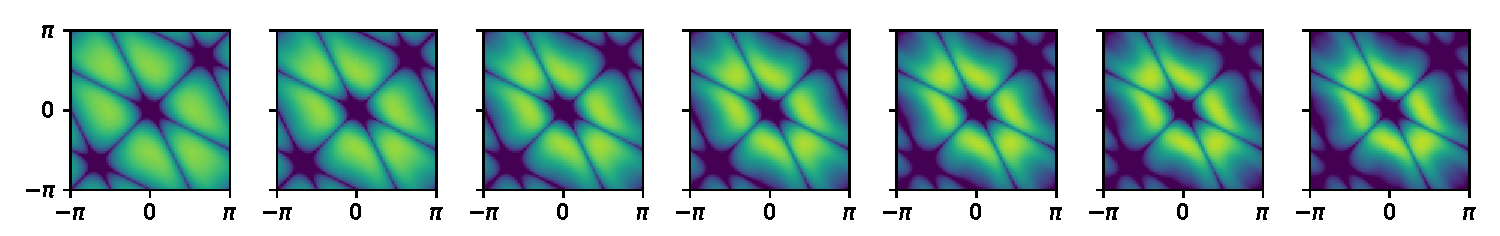
\includegraphics[width=\linewidth]{su3.pdf}
    \vspace{-25pt}
    \caption{ Density of a conjugation equivariant continuous flow on SU(3) in angular coordinates along flow time. Left: Initial distribution according to the Haar-measure. Right: Final distribution approximating the target. Images in between are snapshots at intermediate flow-times.}
    \label{fig:su3}
    \vspace{-10pt}
\end{figure}

\textbf{\color{royalblue}{Future Directions.}}
Leveraging my network of active collaborators, I will address the problem of scaling up to larger lattice sizes, including exploring multi-scale generation, transfer learning, and the thermodynamic properties of these flows. Leveraging the structural overlap in mathematical concepts, I have also recently become excited about the prospect of combining my experience in the context of Calabi-Yau manifolds to improve sampling for $\mathbb{CP}^N$ models, which suffers from topological freezing. This issue is also encountered in gauge theories such as QCD, for which $\mathbb{CP}^N$ serves as a simpler toy model.

I also aim to explore connections between flow-based sampling methods and inverse renormalization group (RG) techniques, which have shown promise in spin glass models. This connection is particularly relevant for scaling up to larger lattice sizes and understanding multi-scale properties, a shared challenge across lattice QCD and condensed matter systems.

Modelling high-dimensional distributions and states with complex correlations between degrees of freedom is a recurring challenge in many fields, from statistical physics to inference problems and condensed matter physics.
This suggests a wide potential for collaborations and a fruitful transfer of ideas between disciplines.
In particular, modeling quantum wavefunctions using techniques similar to generative models has shown success in fields such as quantum chemistry and many-body systems. Exploiting the technological overlap, I hope to extend our methods developed for generative models to explore neural wavefunctions for lattice QCD.


\paragraph{\textit{{Calabi-Yau Metrics.}}}
Calabi-Yau manifolds play a crucial role in string compactifications.
Their geometric structure encoded in the metric is not known analytically, but is required for example to determine the Yukawa couplings of the low-energy effective theory.
This led me to devise novel machine learning methods to approximate Ricci-flat metrics on these manifolds.
By expressing a spectral ansatz that inherently guarantees important differential properties as a trainable neural network, I achieved higher accuracies than established methods more efficiently by simultaneously learning their moduli dependence.
This was made possible by my efficient numerical implementation of intricate mathematical structures such as sections of holomorphic line bundles on complex projective spaces, metrics in local coordinate patches and derived geometric properties like the Ricci curvature.
Building on initial work during my MSc in theoretical and mathematical physics at the LMU Munich, I have since published a library of these computational methods \cite{gerdes2023CYJAXPackage} and co-authored an influential article explaining different machine learning approaches to this problem in collaboration with international collaborators \cite{anderson2021ModulidependentCalabiYau}.

\textbf{\color{royalblue}{Future Directions.}}
A rich space of mathematical constructions of Calabi-Yau manifolds remains to be explored, including the extension of my spectral method to complete intersection Calabi-Yau manifolds.
The field of AI applications in string theory and mathematics is becoming increasingly rich.
In this context, it appears to me that the utilization of long-established ideas in metaheuristics such as particle swarm optimization, simulated annealing and evolutionary algorithms remain under-explored.
I therefor aim to investigate, in particular, how these methods may be leveraged in the context of conformal bootstrap and the search for string vacua.


\paragraph{\textit{{Interdisciplinary Research Bridging Theory and Computation.}}}
Informed by my work on generative models for lattice quantum field theory, I have explored connections between RG and diffusion models.
This led me to develop a generalized RG-inspired framework for diffusion models \cite{gerdes2024gudgenerationunifieddiffusion}, in collaboration with Prof Max Welling, that enlarges the design space for diffusive processes and makes explicit its sequential nature.

Another example of interdisciplinary work I have enjoyed is in statistical data analysis and in particular simulation based inference, which incorporates machine learning to tackle large numbers of nuisance parameters that can arise from more faithful physical models.
Stellar streams are a probe for the structure of the Milky Way and in particular for the sub-halo distribution of dark matter with which they may interact gravitationally. Constraining theoretical properties of interest from a particular observations leads to a statistical inference problem due to the complexity of their relation as well as presence of uncertainty and nuisance parameters.
Given a statistical model as a sampler which can probabilistically simulate observations given a set of theory parameters, simulation based inference leverages machine learning to find the Bayesian posterior distribution for parameters of interest.
This allows for a large numbers of nuisance parameters that can arise from more faithful physical models and significantly improves on traditional Monte Carlo methods in terms of efficiency.
I have implemented a performant simulator for stellar streams evolving in a gravitational background, and implemented a simulation based inference pipeline using neural ratio estimation \cite{alvey2023AlbatrossScalable}, laying the groundwork for future theoretical insights derived from astrophysical observations.

This work on statistical inference led me to study theoretical statistics and differences between frequentist and Bayesian approaches in this field.
Having discovered an interesting dual point of view between these, I am presently developing optimization schemes that combine and unify notions from both frequentism and Bayesianism.


\bibliographystyle{abbrvnat-sorted}
{
    \small
    \bibliography{refs}
}

\end{document}
